\documentclass[12pt]{article}
\usepackage{amsmath}
\usepackage{amssymb}
\usepackage{enumerate}
\usepackage{geometry}
\usepackage{tikz}
\usetikzlibrary{automata, positioning, arrows}
\geometry{margin=1in}

\title{Problem Set 4 - CPSC 326\\Solutions}
\author{Fernando, Dang, Raj, Eric M.}
\date{\today}

\begin{document}
\maketitle

\section*{Problem 1}
Consider the following Language:
$$L_1 = \{w \in \{a, b, c, d\}^* \mid (w \text{ contains the strings } abb \text{ and } bbc) \text{ or } (w \text{ contains the string } abc)\}$$

Develop a NFA for $L_1$.

\textbf{Answer:}

The NFA uses nondeterminism to check for either:
\begin{itemize}
    \item Case 1: Both $abb$ and $bbc$ appear in $w$
    \item Case 2: $abc$ appears in $w$
\end{itemize}

\textbf{States:}
\begin{itemize}
    \item $q_0$: Initial state
    \item $q_1, q_2, q_3$: Track progress toward finding $abb$
    \item $q_4, q_5, q_6$: Track progress toward finding $bbc$ (after finding $abb$)
    \item $q_7$: Found both $abb$ and $bbc$ (accepting)
    \item $q_8, q_9, q_{10}$: Track progress toward finding $abc$
    \item $q_{11}$: Found $abc$ (accepting)
\end{itemize}

\textbf{NFA Diagram:}

\begin{center}
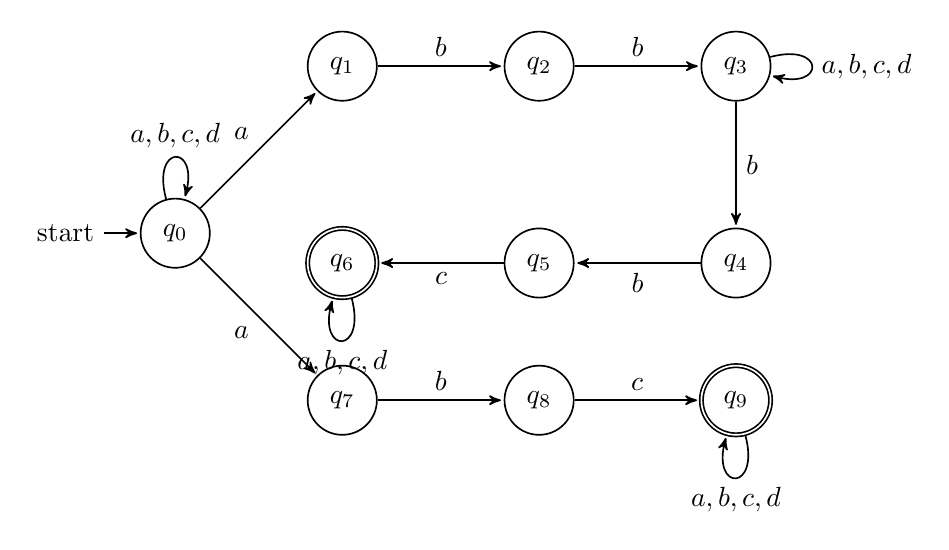
\begin{tikzpicture}[>=stealth', shorten >=1pt, auto, node distance=2.5cm, semithick]
    % Initial state
    \node[state, initial] (q0) {$q_0$};
    
    % Path for abb
    \node[state] (q1) [above right of=q0, node distance=3cm] {$q_1$};
    \node[state] (q2) [right of=q1] {$q_2$};
    \node[state] (q3) [right of=q2] {$q_3$};
    
    % Path for bbc (after abb)
    \node[state] (q4) [below of=q3] {$q_4$};
    \node[state] (q5) [left of=q4] {$q_5$};
    \node[state, accepting] (q6) [left of=q5] {$q_6$};
    
    % Path for abc
    \node[state] (q7) [below right of=q0, node distance=3cm] {$q_7$};
    \node[state] (q8) [right of=q7] {$q_8$};
    \node[state, accepting] (q9) [right of=q8] {$q_9$};
    
    \path[->]
    % Self-loop on start
    (q0) edge [loop above] node {$a,b,c,d$} (q0)
    
    % Path to find abb
    (q0) edge node [above left] {$a$} (q1)
    (q1) edge node {$b$} (q2)
    (q2) edge node {$b$} (q3)
    (q3) edge [loop right] node {$a,b,c,d$} (q3)
    
    % From q3, find bbc
    (q3) edge node [right] {$b$} (q4)
    (q4) edge node {$b$} (q5)
    (q5) edge node {$c$} (q6)
    (q6) edge [loop below] node {$a,b,c,d$} (q6)
    
    % Path to find abc directly
    (q0) edge node [below left] {$a$} (q7)
    (q7) edge node {$b$} (q8)
    (q8) edge node {$c$} (q9)
    (q9) edge [loop below] node {$a,b,c,d$} (q9);
\end{tikzpicture}
\end{center}

\textbf{Explanation:}
The NFA nondeterministically chooses between:
\begin{itemize}
    \item Following the upper path to find $abb$, then continuing to find $bbc$
    \item Following the lower path to find $abc$
\end{itemize}
Once either accepting state is reached, the string is accepted.

\newpage

\section*{Problem 2}
Let $L_2 = \{w \in \{a, b, c\}^* \mid w = (abc)^*a^*\}$. Design a NFA that accepts the language $L_2$.

\textbf{Answer:}

The language consists of zero or more repetitions of $abc$, followed by zero or more $a$'s.

\textbf{States:}
\begin{itemize}
    \item $q_0$: Initial and accepting state
    \item $q_1$: Just read $a$ (could be start of $abc$ or final $a$'s)
    \item $q_2$: Read $ab$ (continuing $abc$)
    \item $q_3$: Read $abc$ (back to accepting, or continue with more $a$'s)
\end{itemize}

\textbf{NFA Diagram:}

\begin{center}
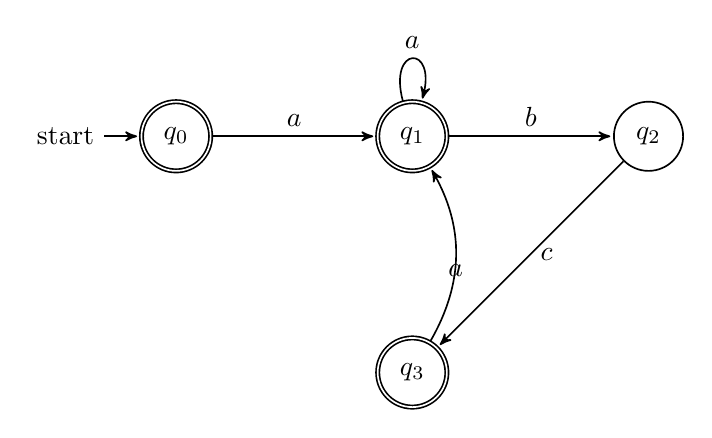
\begin{tikzpicture}[>=stealth', shorten >=1pt, auto, node distance=3cm, semithick]
    \node[state, initial, accepting] (q0) {$q_0$};
    \node[state, accepting] (q1) [right of=q0] {$q_1$};
    \node[state] (q2) [right of=q1] {$q_2$};
    \node[state, accepting] (q3) [below of=q1] {$q_3$};
    
    \path[->]
    (q0) edge node [above] {$a$} (q1)
    (q1) edge node [above] {$b$} (q2)
    (q2) edge node [right] {$c$} (q3)
    (q3) edge [bend right=30] node [below] {$a$} (q1)
    (q1) edge [loop above] node {$a$} (q1);
\end{tikzpicture}
\end{center}

\textbf{Explanation:}
\begin{itemize}
    \item From $q_0$, we can either accept immediately ($\varepsilon$ is in the language) or read $a$
    \item After reading $a$, we nondeterministically choose:
    \begin{itemize}
        \item Continue with $bc$ to complete an $abc$ block
        \item Stay in $q_1$ reading more $a$'s (the final $a^*$ part)
    \end{itemize}
    \item After completing $abc$ (reaching $q_3$), we can start another $abc$ block or accept
    \item States $q_0$, $q_1$, and $q_3$ are accepting to handle $(abc)^*a^*$ properly
\end{itemize}

\newpage

\section*{Problem 3}
Let $L_3 = \{w \in \{0, 1, 2, 3, 4, 5, 6, 7, 8, 9\}^* \mid \text{the final digit of the string } w \text{ has not appeared before in } w\}$.

Design a NFA that accepts the language $L_3$.

\textbf{Answer:}

The NFA uses nondeterminism to guess which digit will be the final digit that hasn't appeared before.

\textbf{Strategy:}
From the start state, when we read symbols, we nondeterministically choose which digit we're "watching for" as the final new digit. We have 10 branches (one for each digit 0-9), where each branch avoids seeing that specific digit until the very end.

\textbf{States:}
\begin{itemize}
    \item $q_0$: Initial state (accepting, for single-digit strings)
    \item Branches for each digit:
    \begin{itemize}
        \item $q_1, q_2$: Branch watching for digit 0
        \item $q_3, q_4$: Branch watching for digit 1
        \item $q_5, q_6$: Branch watching for digit 2
        \item $q_7, q_8$: Branch watching for digit 3
        \item $q_9, q_{10}$: Branch watching for digit 4
        \item $q_{11}, q_{12}$: Branch watching for digit 5
        \item $q_{13}, q_{14}$: Branch watching for digit 6
        \item $q_{15}, q_{16}$: Branch watching for digit 7
        \item $q_{17}, q_{18}$: Branch watching for digit 8
        \item $q_{19}, q_{20}$: Branch watching for digit 9
    \end{itemize}
    \item Accepting states: $q_0, q_2, q_4, q_6, q_8, q_{10}, q_{12}, q_{14}, q_{16}, q_{18}, q_{20}$
\end{itemize}

\textbf{NFA Diagram:}

\begin{center}
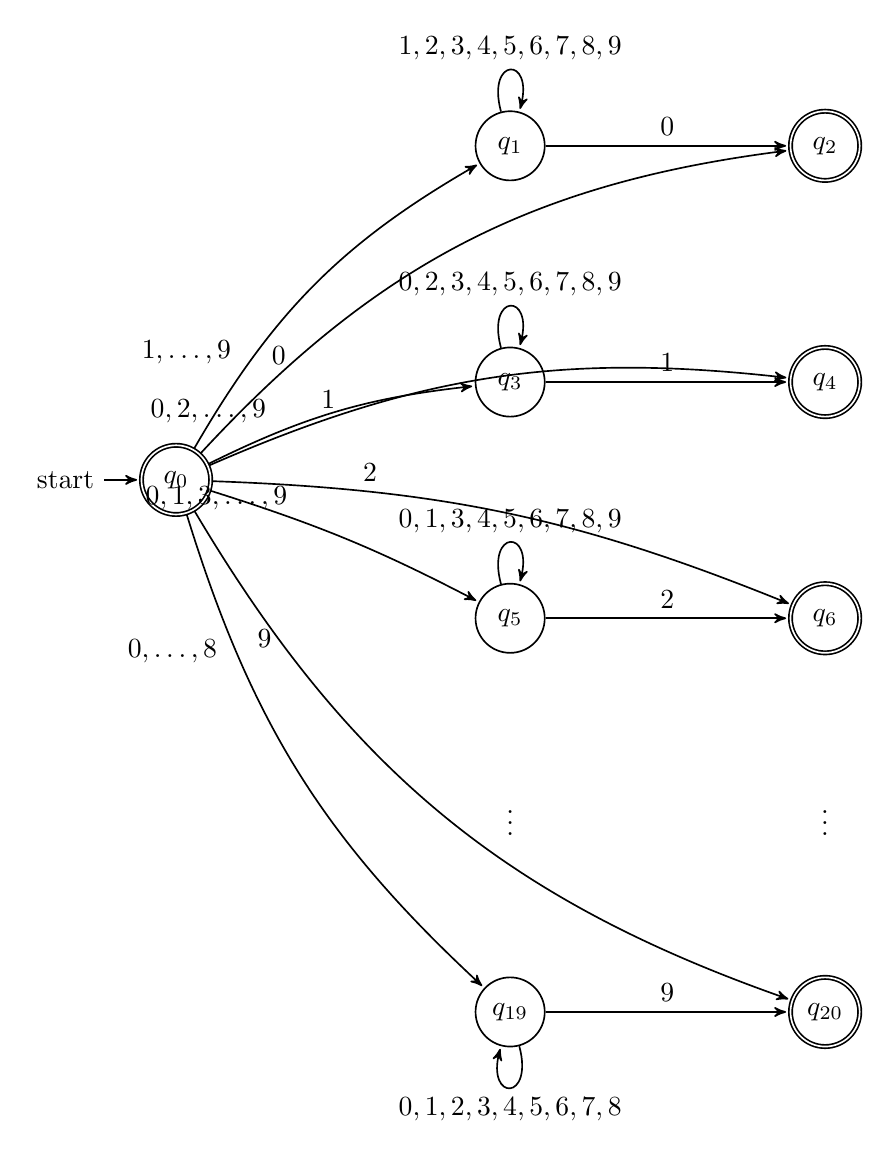
\begin{tikzpicture}[>=stealth', shorten >=1pt, auto, node distance=5cm, semithick]
    \node[state, initial, accepting] (q0) {$q_0$};
    
    % Branch for watching digit 0: q1 -> q2
    \node[state] (q1) [above right of=q0, node distance=6cm] {$q_1$};
    \node[state, accepting] (q2) [right of=q1, node distance=4cm] {$q_2$};
    
    % Branch for watching digit 1: q3 -> q4
    \node[state] (q3) [below of=q1, node distance=3cm] {$q_3$};
    \node[state, accepting] (q4) [right of=q3, node distance=4cm] {$q_4$};
    
    % Branch for watching digit 2: q5 -> q6
    \node[state] (q5) [below of=q3, node distance=3cm] {$q_5$};
    \node[state, accepting] (q6) [right of=q5, node distance=4cm] {$q_6$};
    
    % Dots to indicate more branches
    \node (dots1) [below of=q5, node distance=2.5cm] {$\vdots$};
    \node (dots2) [below of=q6, node distance=2.5cm] {$\vdots$};
    
    % Branch for watching digit 9: q19 -> q20
    \node[state] (q19) [below of=dots1, node distance=2.5cm] {$q_{19}$};
    \node[state, accepting] (q20) [right of=q19, node distance=4cm] {$q_{20}$};
    
    \path[->]
    % Branch for digit 0 (q1 -> q2)
    (q0) edge [bend left=15] node [above left, pos=0.2] {$1,\ldots,9$} (q1)
    (q0) edge [bend left=20] node [above, pos=0.15] {$0$} (q2)
    
    % q1: reading non-0 digits, watching for 0
    (q1) edge [loop above] node {$1,2,3,4,5,6,7,8,9$} (q1)
    (q1) edge node [above] {$0$} (q2)
    
    % Branch for digit 1 (q3 -> q4)
    (q0) edge [bend left=10] node [above left, pos=0.25] {$0,2,\ldots,9$} (q3)
    (q0) edge [bend left=15] node [above, pos=0.2] {$1$} (q4)
    
    % q3: reading non-1 digits, watching for 1
    (q3) edge [loop above] node {$0,2,3,4,5,6,7,8,9$} (q3)
    (q3) edge node [above] {$1$} (q4)
    
    % Branch for digit 2 (q5 -> q6)
    (q0) edge [bend left=5] node [above left, pos=0.3] {$0,1,3,\ldots,9$} (q5)
    (q0) edge [bend left=10] node [above, pos=0.25] {$2$} (q6)
    
    % q5: reading non-2 digits, watching for 2
    (q5) edge [loop above] node {$0,1,3,4,5,6,7,8,9$} (q5)
    (q5) edge node [above] {$2$} (q6)
    
    % Branch for digit 9 (q19 -> q20)
    (q0) edge [bend right=15] node [below left, pos=0.2] {$0,\ldots,8$} (q19)
    (q0) edge [bend right=20] node [below, pos=0.15] {$9$} (q20)
    
    % q19: reading non-9 digits, watching for 9
    (q19) edge [loop below] node {$0,1,2,3,4,5,6,7,8$} (q19)
    (q19) edge node [above] {$9$} (q20);
\end{tikzpicture}
\end{center}

\textbf{Explanation:}

The NFA has 21 states total ($q_0$ through $q_{20}$), organized as follows:
\begin{itemize}
    \item $q_0$: Starting state (also accepting for single-digit strings)
    \item 10 branches, each with 2 states, one for each digit 0-9:
    \begin{itemize}
        \item States $q_1, q_3, q_5, q_7, q_9, q_{11}, q_{13}, q_{15}, q_{17}, q_{19}$: "Avoiding" states where we read any digit except the one we're watching for
        \item States $q_2, q_4, q_6, q_8, q_{10}, q_{12}, q_{14}, q_{16}, q_{18}, q_{20}$: "Found" states (accepting) where we just read the digit we were watching for
    \end{itemize}
\end{itemize}

How it works:
\begin{enumerate}
    \item From $q_0$, nondeterministically choose which digit will be the final new digit
    \item For example, to watch for digit 0:
    \begin{itemize}
        \item Go to $q_1$ by reading any digit 1-9
        \item Stay in $q_1$ reading more digits 1-9 (avoiding 0)
        \item Read 0 and go to accepting state $q_2$
    \end{itemize}
    \item Similarly for digits 1-9, using states $(q_3, q_4), (q_5, q_6), \ldots, (q_{19}, q_{20})$
\end{enumerate}

\textbf{Example:}

For string $w = 237$ (where 7 appears for the first time at the end):
\begin{itemize}
    \item Read 2: $q_0 \xrightarrow{2} q_{15}$ (nondeterministically choose to watch for 7)
    \item Read 3: $q_{15} \xrightarrow{3} q_{15}$ (3 is not 7, stay in $q_{15}$)
    \item Read 7: $q_{15} \xrightarrow{7} q_{16}$ (accept!)
\end{itemize}

For string $w = 5$ (single digit):
\begin{itemize}
    \item Read 5: $q_0 \xrightarrow{5} q_{12}$ (accept immediately)
    \item Or stay in $q_0$ which is also accepting
\end{itemize}

\end{document}